%!TEX root = practicum1.tex
We have fixed the value of $K$ to 1, essentially removing the parameter from the equation. By choosing different initial values we can generate three different types of orbits: zero-, one- and two-dimensional. The three orbit types are discussed in respectively \cref{sss:experiment:a:discrete}, \ref{sss:experiment:a:closed} and \ref{sss:experiment:a:2D}.

 	\begin{figure}
		\centering
		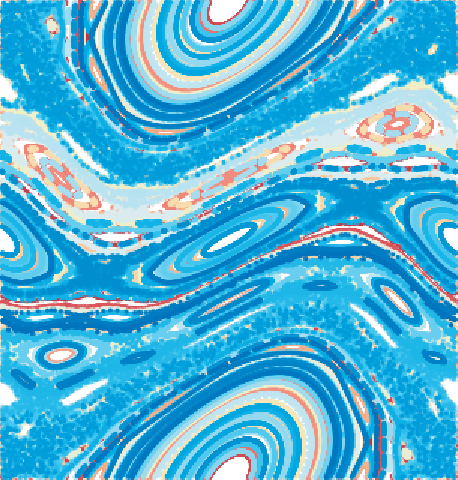
\includegraphics[width=0.9\columnwidth, height=0.2\textheight, keepaspectratio=true]{./img/assignment_a_pretty_low_res.pdf}
		\caption{Phase-space diagram, $p_n$ as a function of $x_n$, of 500 randomly initialized orbits of the Chirikov map for $K = 1$, with $0 \leq n \leq 1000$, and $x_0$ and $p_0$ in the unit square.}
		\label{fig:a:pretty}
	\end{figure}

\subsubsection{Discrete Points}
\label{sss:experiment:a:discrete}
Zero-dimensional orbits consist of a finite number of points, which are found in the centres of the islands in \cref{fig:a:pretty} \cite{kenzel1997physics}. We first discuss a specific initialization that results in such an orbit, before moving to the general case.\\

We have generated a zero-dimensional Chirikov map by choosing $x_0 = p_0 = 0.5$. Using these values $p_1 = p_0$ since the second term of \eqref{eq:chirikov:p} becomes zero. This results in
\begin{equation*}
	x_1 = \left( x_0 + p_{1} \right) \mod 1= 0.	
\end{equation*}
The next steps of the map, for $n > 0$, are easily derived since $p_{n + 1}$ will not change due to the fact that both 0 and 0.5 as input to \eqref{eq:chirikov:p} result in the second term becoming zero. 

With the initialization $\left\{x_0\,, p_0 \right\} = \{{0.5},\,{0.5}\}$, $x_{n} \in \left\{0,\, 0.5 \right\} \text{ for } n \geq 0$. To illustrate $x_2$ is $0.5 + 0 = 0.5$ which is equal to $x_1$. We have now shown that $p_n$ is constant for $n \geq 1$ and that $x_n$ jumps between 0 and 0.5, which is illustrated in \cref{fig:experiment:dimension:0:p} and \cref{fig:experiment:dimension:0:x}. This conclusion also explains the phase space diagram, \cref{fig:experiment:dimension:0}, and the plot in \cref{fig:experiment:dimension:0:t}. 

Furthermore we have shown that these points are visited in a fixed order.\\

From this specific initialization we can derive the following constraints for $p_0$ and $x_0$; $x_0$ should be chosen in such a way that the sine in \cref{eq:chirikov:p} becomes 0, i.e. $x_0 \in \{0,\, 0.5,\, 1\}$. Due to the constraint on $x_0$,
\begin{equation*}
p_{n + 1} = \left( p_{n} \mod 1 \right),
\end{equation*}
	which is equal to $p_n$, unless $p_n = 1$. Consequently
	\begin{equation*}
	x_{n + 1} = \left( x_n + p_n \mod 1 \right),
	\end{equation*}
unless $p_1 = 1$. Formally, one should choose $p_0$ in such a way that:
\begin{equation*}
	\left( \left[ x_0 + (p_0 \mod 1)\right] \mod 1 \right) \in \left\{0, 0.5, 1\right\}.
\end{equation*}

\subsubsection{Closed curves}
\label{sss:experiment:a:closed}
One-dimensional orbits are represented in the phase-space diagram in \cref{fig:a:pretty} as the closed curves around the islands formed by the zero-dimensional orbits.

We have determined empirically that $\left\{x_0\,, p_0 \right\} = {\num{0.1576131},\,\num{0.9705928}}$ results in closed curves. \Cref{fig:experiment:dimension:1} shows $p_n$ as a function of $x_n$, \cref{fig:experiment:dimension:1:p} and \ref{fig:experiment:dimension:1:x} show the progression of respectively $p$ and $x$.\\

Considering these figures we see that the progression of both $p$ and $x$ happens according to a fixed pattern with a seemingly periodic shift. Examining \cref{fig:experiment:dimension:1:t} we see that $x$, the orange dashed line, slowly moves from one extreme to the other, which is reflected in \cref{fig:experiment:dimension:1:x}. Considering $p$ in \cref{fig:experiment:dimension:1:t}, the solid blue line, we find that its value moves between approximately 0.2 and 0.8, and then oscillates around that value before going back to the other value. This is represented in \cref{fig:experiment:dimension:1:p} by the high density areas in the lower left and upper right corners.

\begin{figure}
	\centering
	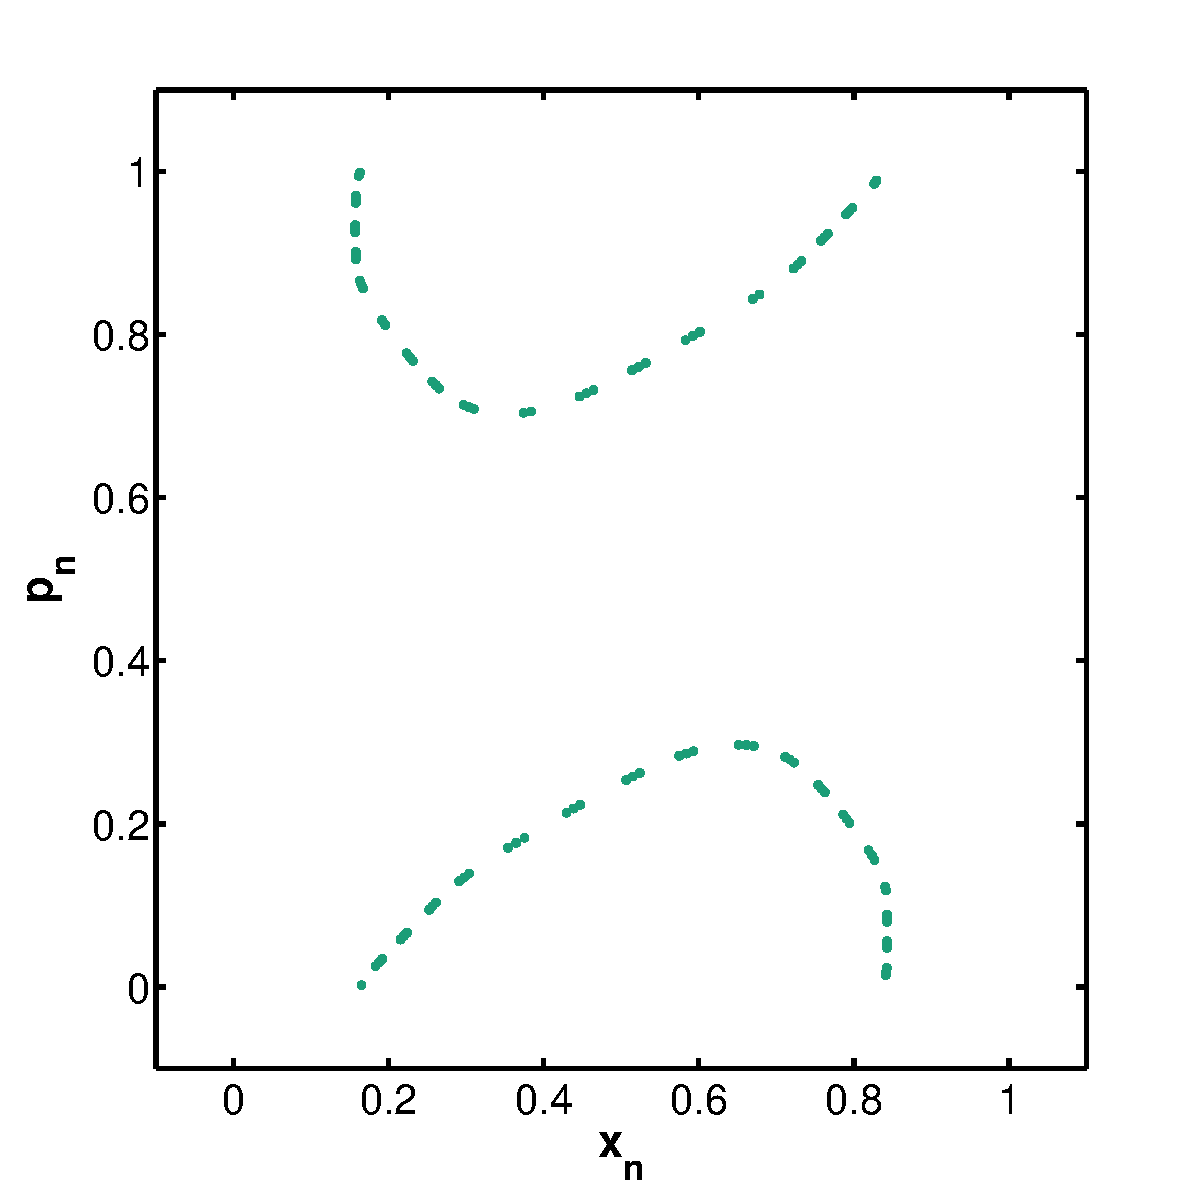
\includegraphics[width=0.9\columnwidth]{./img/assignment_a_1_dim_n100}
	\caption{$p_n = \num{0.1576131}$ as a function of $x_n= \num{0.9705928}$, for $n = 100$.}
	\label{fig:experiment:a_1_n100}
\end{figure}

%!TEX root = practicum1.tex

\begin{figure*}
	\centering
	% \x/\picname in {4/pic1.png,8/pic2.png,15/pic3.png,16/pic4.png}
	\foreach \dim/\x/\p in {0/0.500/0.500, 1/0.1576131/0.9705928, 2/0.1269868/0.9133759}
	{ 
		\begin{subfigure}[t]{0.32\textwidth}
			\includegraphics[width=\textwidth]{./img/assignment_a_\dim_dim.pdf}
			\caption{$x_0=\num{\x}$, $p_0=\num{\p}$}
			\label{fig:experiment:dimension:\dim}
		\end{subfigure}
		\begin{subfigure}[t]{0.32\textwidth}
			\includegraphics[width=\textwidth]{./img/assignment_a_\dim_dim_progression_p.pdf}
			\caption{Progression of $p$ in \subref{fig:experiment:dimension:\dim}}
			\label{fig:experiment:dimension:\dim:x}
		\end{subfigure}		
		\begin{subfigure}[t]{0.32\textwidth}
			\includegraphics[width=\textwidth]{./img/assignment_a_\dim_dim_progression_x.pdf}
			\caption{Progression of $x$ in \subref{fig:experiment:dimension:\dim}}
			\label{fig:experiment:dimension:\dim:p}
		\end{subfigure}		
	}
	\caption{Each row corresponds to on set of initial values $\left\langle x_0, p_0 \right\rangle$. The first column shows $x_n$ versus $p_n$ for $n \in \left[0,\, \num{10000} \right]$. The second and third column depict respectively the progression of $p$ and $x$.}
	\label{fig:experiment:dimension}
\end{figure*}

We can conclude that the points of \cref{fig:experiment:dimension:1} are visited in a fixed order. Colloquially one could say that the map starts by generating a low density version of \cref{fig:experiment:dimension:1}, see \cref{fig:experiment:a_1_n100}, which is then filled in by iterating over the figure multiple times. Due to the small shift, the area of the closed curve is filled in after a large number of iterations.

\subsubsection{Two-Dimensional Orbits}	
\label{sss:experiment:a:2D}
	Two-dimensional orits fill entire areas by jumping around chaotically. The empirically determined values $\left\{x_0\,, p_0 \right\} = {\num{0.1269868},\,\num{0.9133759}}$ result in an orbit that fills the two-dimensional areas in \cref{fig:experiment:dimension:2}. Comparing \cref{fig:experiment:dimension:1:p} with \cref{fig:experiment:dimension:2:p} we see the same general pattern, however \cref{fig:experiment:dimension:2:p} shows more chaotic behaviour. We observe the same behaviour for $x$ when contrasting \cref{fig:experiment:dimension:1:x} with \cref{fig:experiment:dimension:2:x}. This is supported by comparing \cref{fig:experiment:dimension:1:t} with \cref{fig:experiment:dimension:2:t}, where we find that the blue and orange line have the same trajectory, approximately but that the lines in \cref{fig:experiment:dimension:2:t} change more, and change with a varying value every period.

	Since the map with orbits is essentially the same as the map with the closed curves the single points are also visited in a fixed order. 

	As the values of $p$ and $x$ vary more, we plotting $p$ as a function of $x$ results in an area around the curves that we saw in \cref{fig:experiment:dimension:1}.
